\documentclass[22pt]{beamer}

\usepackage{templates/beamerthemekit}
\usepackage{graphicx}
\usepackage[utf8]{inputenc}
\usepackage[ngerman]{babel}

\title[OSIP]{OPC UA Simulator for Industrial Plants}
\subtitle{PSE Projekt}
\author{M. Armbruster, D. Kahles, H. Lehmann, M. Schwarzmann, N. Wilhelm}

\titlelogo{icon}

\begin{document}

\selectlanguage{ngerman}

%title page
\begin{frame}
\titlepage
\end{frame}

\begin{frame}{Wofür benötigt man OSIP?}
\begin{figure}[ht!]
\centering
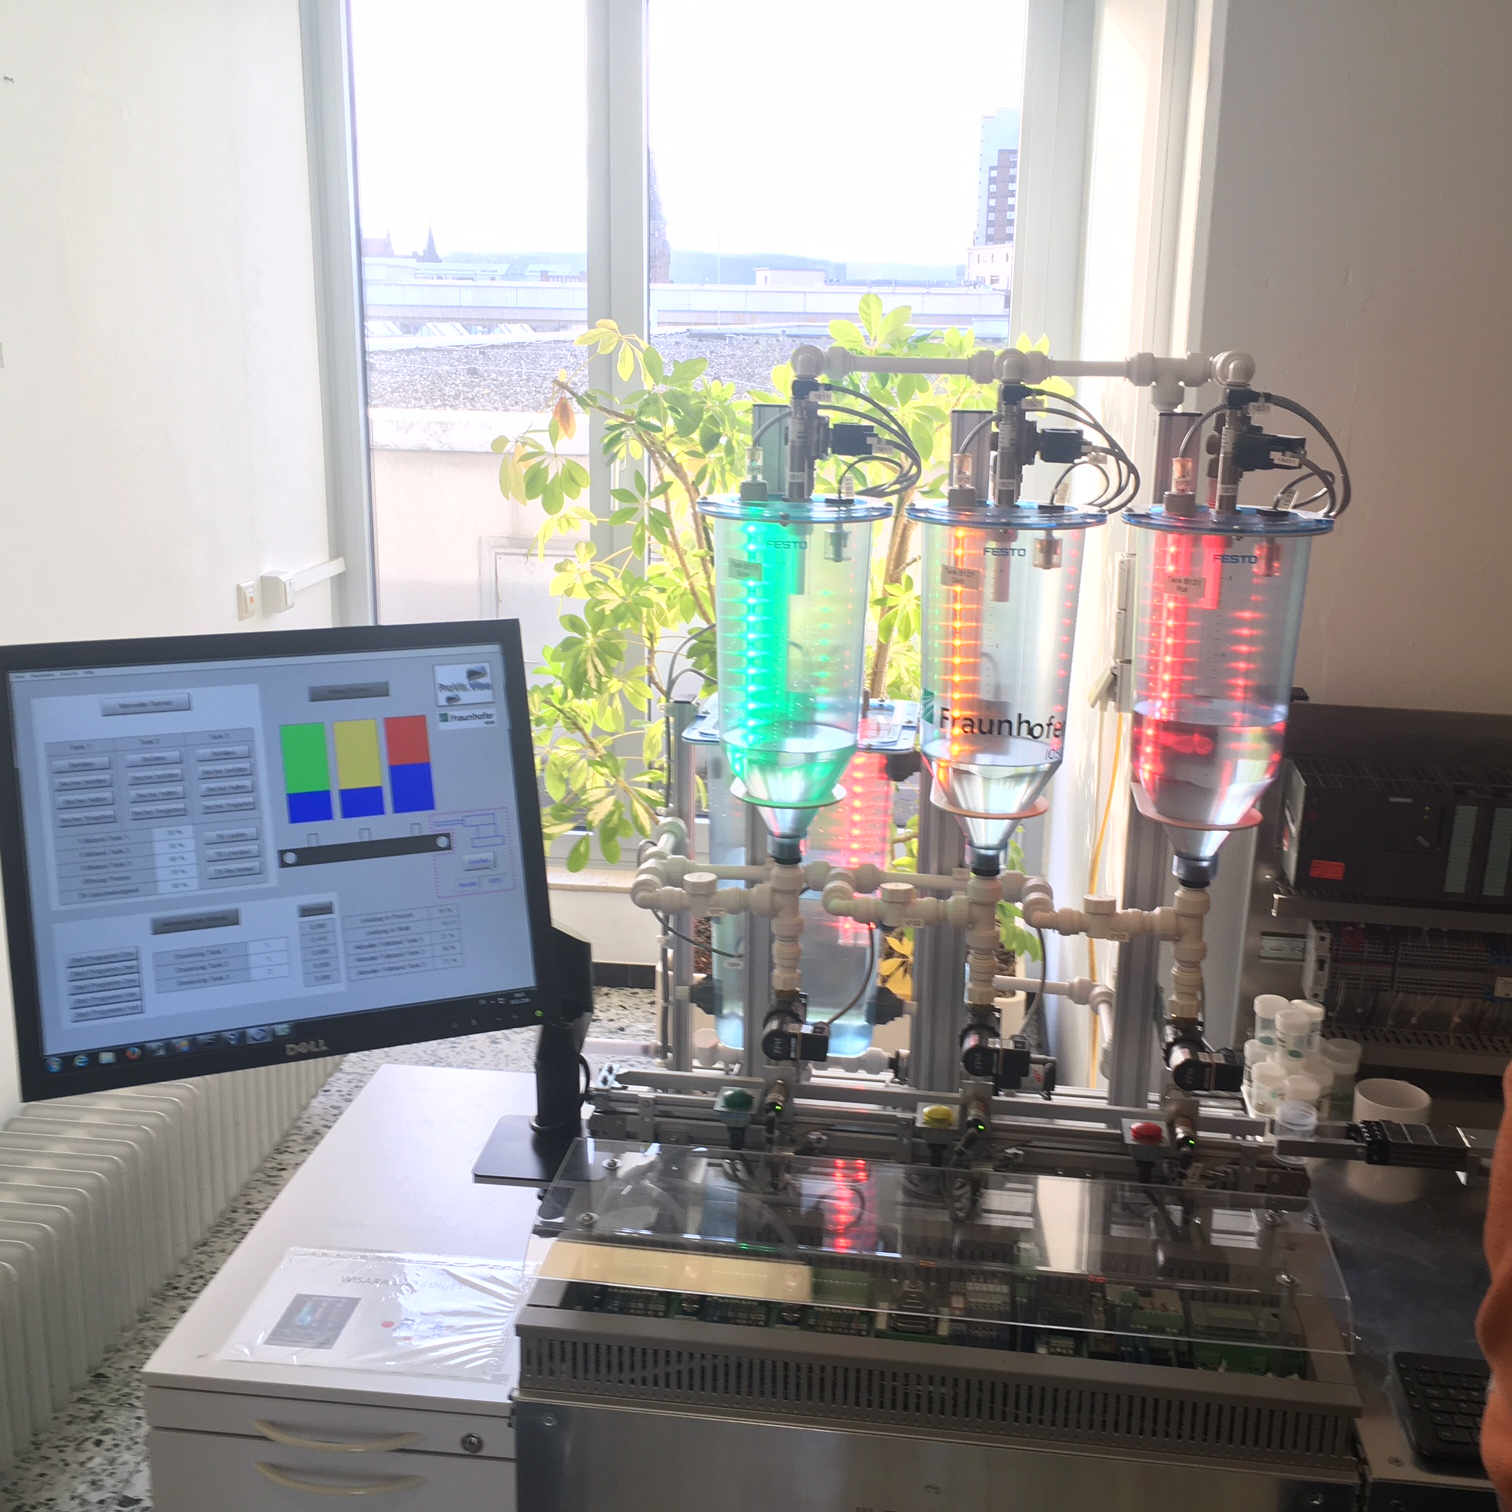
\includegraphics[height=\textheight,width=\textwidth,keepaspectratio=true]{Demoanlage_IOSB.jpg}
\end{figure}
\end{frame}

\begin{frame}{Was ist OSIP?}
\begin{itemize}[<+->]
 \item zwei Anwendungen: \emph{Simulation} eines chemischen Produktionsprozesses mit vier Tanks und \emph{Überwachungskonsole}
 \item Kommunikation ausschließlich über OPC UA Protokoll
 \item Anwendungen per Netzwerk auf getrennten Computern lauffähig
\end{itemize}
\end{frame}

\begin{frame}{Simulation}
\vspace*{-1em}
 \begin{center}
 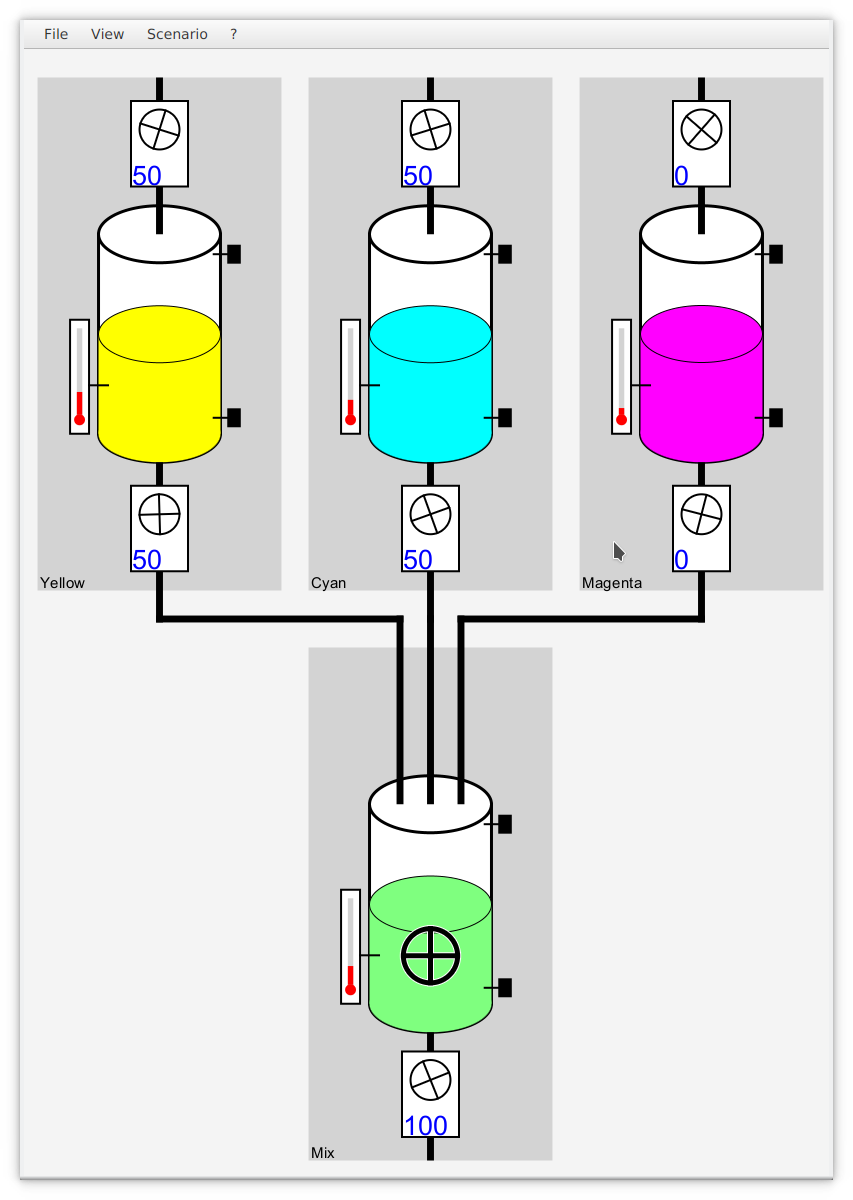
\includegraphics[height=0.9\textheight,width=0.9\textwidth,keepaspectratio=true]{ScreenshotSimulation.png}
 \end{center}
\end{frame}

\begin{frame}{Überwachungskonsole}
  \vspace*{-1em}
 \begin{center}
  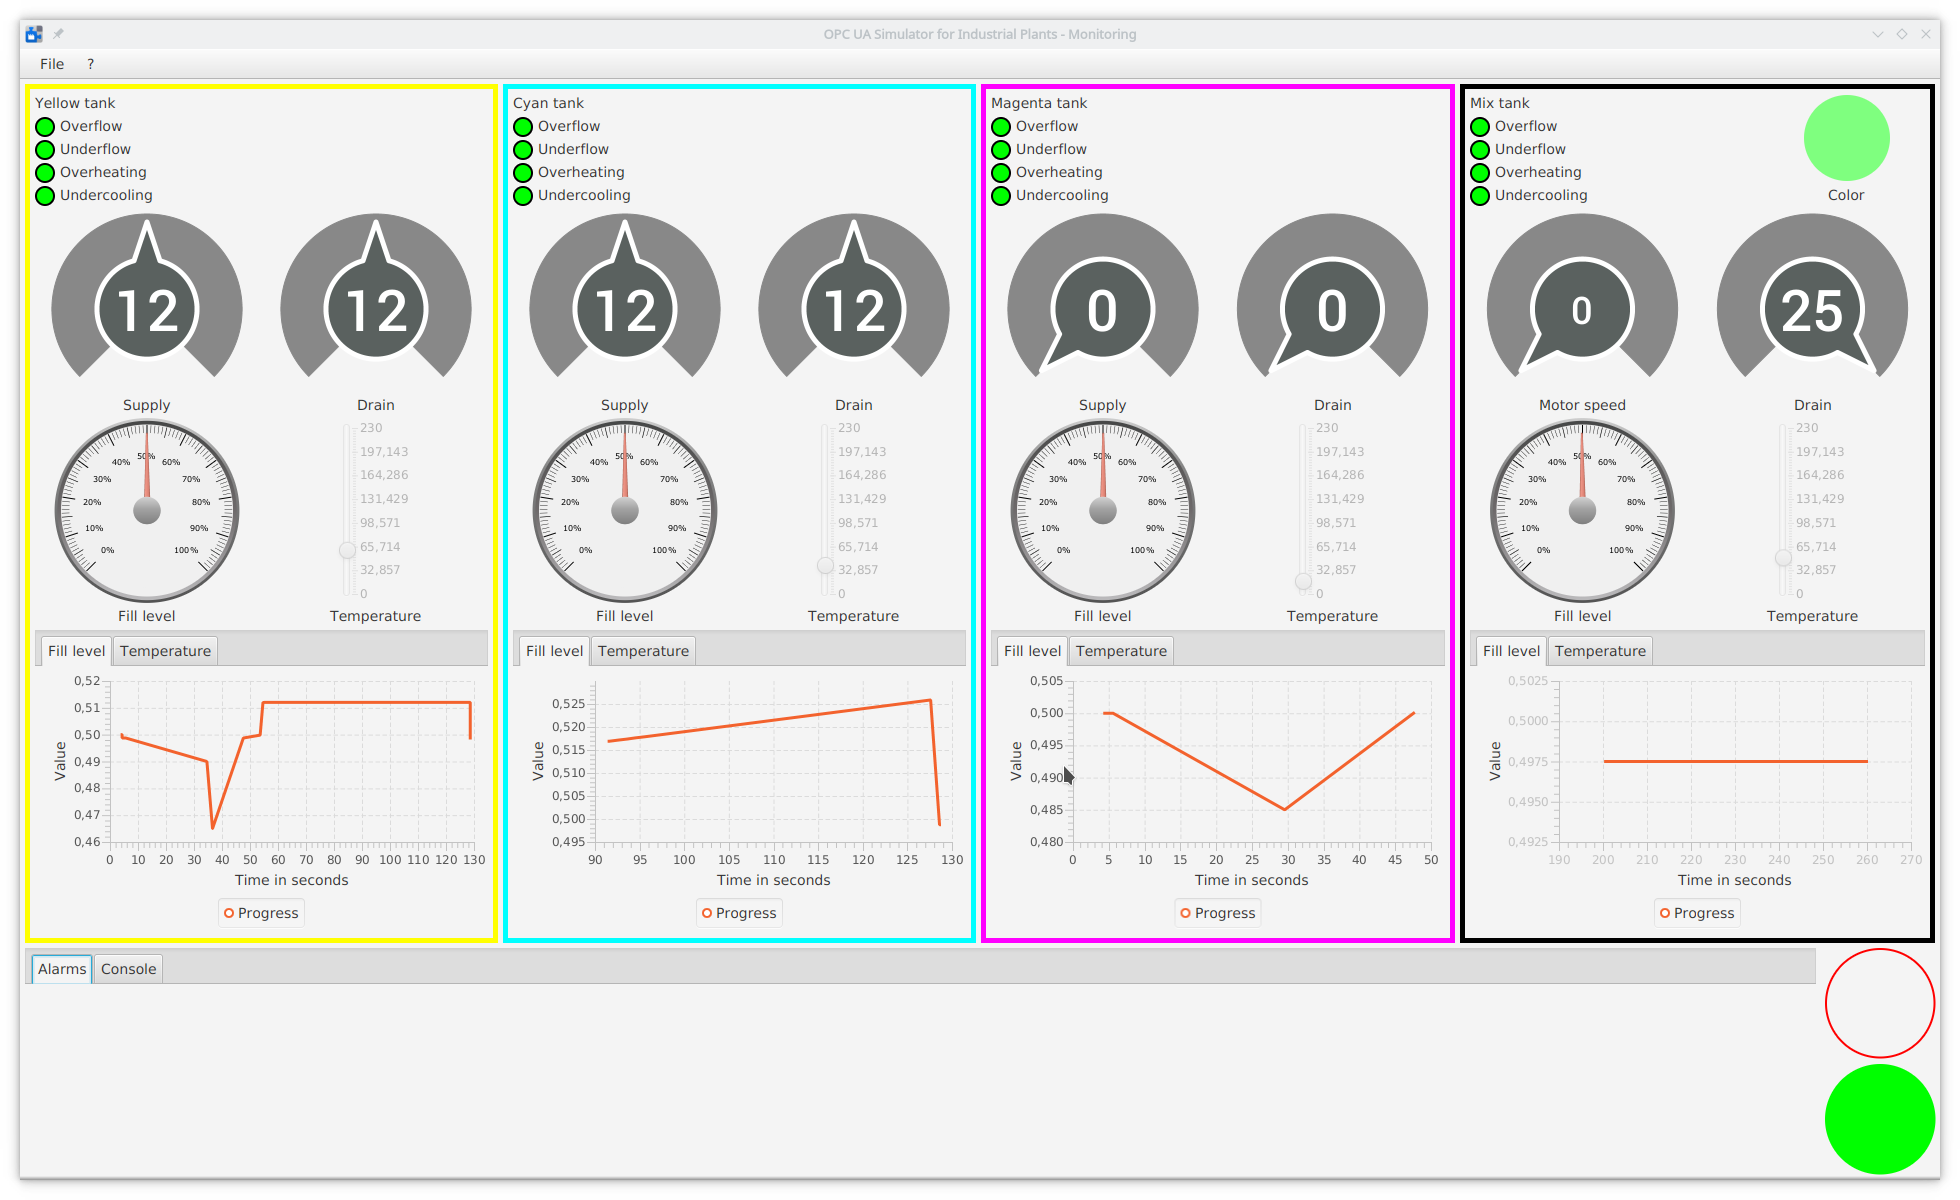
\includegraphics[height=0.9\textheight,width=0.9\textwidth,keepaspectratio=true]{ScreenshotMonitor.png}
 \end{center}
\end{frame}

\begin{frame}{Verwendete Technologien}
\begin{itemize}[<+->]
 \item OPC UA Protokoll nicht selbst implementieren $\rightarrow$ Open Source Implementierung \emph{Milo}
 \item Programmiersprache: \emph{Java}
 \item Bauen des Projekts: \emph{Maven}
 \item Entwicklung der GUI: \emph{JavaFX}
 \item \emph{Git} (circa 800 Commits), Codereview und CI auf \emph{GitHub.com}
 \item Plattformen: Ubuntu 16.04 und Windows 10
 \item Unter Ubuntu: einfaches starten in Docker Containern
 \item Verschiedene Entwurfsmuster (MVC, Beobachter, Fassade, Strategie, ...)
 \item Circa 15.000 LOC, davon 7500 SLOC
\end{itemize}
\end{frame}

\begin{frame}{It's Showtime}
\centering
\huge
\textbf{Demo}
\end{frame}

\begin{frame}{Resümee}
\begin{itemize}[<+->]
 \item Code Review vermeidet viele Probleme
 \item Controller aufwändiger als gedacht
 \item Unittesten der Nicht-GUI Komponenten nützlich
 \item Zeitplan dank Puffer bisher eingehalten
 \item Fast alle geplanten Features umgesetzt
\end{itemize}
\end{frame}

\end{document}
